Das Ziel von der Port und Adapter Architektur ist die Logik (das Verhalten) der Anwendung von
den benutzen Schnittstellen zu trennen. Damit können die externen Schnittstellen schnell und problemlos ausgetauscht werden und
es besteht die Möglichkeit die Anwendung ohne Schnittstellen zu starten. 

Laut der Architekturbeschreibung besteht die Anwendung, die nach der Ports und Adapters Architektur umgesetzt ist, aus drei wesentliche Teile:
\begin{itemize}
    \item Ports (blaues Teil)
    \item Adapters (rotes Teil)
    \item Core (gelbes Teil)
\end{itemize}

Im \textbf{Core} ist das komplette Verhalten der Anwendung definiert.
Jeder \textbf{Port} verbindet die Anwendung mit einer anderen externen Anwendung (z.B. Benutzeroberfläche wird über HTTP-Schnittstelle verbunden oder Datenbank-Schnittstelle).
Jeder \textbf{Port} benötigt einen \textbf{Adapter}, um die ankommenden Nachrichten für den \textbf{Core} zu transformieren bzw. 
ausgehende Nachrichten für den \textbf{Port} zu transformieren.\cite{portAndAdapter}

\begin{figure}[H]
    \centering
    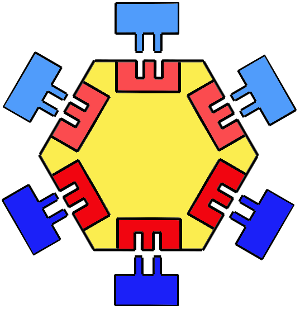
\includegraphics[width=0.7\textwidth]{./images/ports-and-adapters.png}
    \caption[Port und Adapter Architektur]{Port und Adapter Architektur \footnotemark}
    \label{fig:PortAndAdapterArchitecture}
\end{figure}
\footnotetext{$https://www.dossier-andreas.net/software_architecture/ports_and_adapters.html$}